% Research proposal distilled from the November 2026 technical backbone.
% !TeX program = xelatex
% Standalone source: XeLaTeX (Hebrew title), no external graphics or bibliography files.
% The accompanying backbone/research_backbone.pdf preserves the full technical record.
% Public output: research_proposal.pdf; run build_documents.ps1.
\documentclass[11pt,a4paper]{article}
\usepackage{fontspec}
\newfontfamily\hebrewtitlefont[Script=Hebrew]{Arial}
\usepackage[english]{babel}
\usepackage{lmodern}
\usepackage[margin=0.92in,headheight=15pt]{geometry}
\usepackage{amsmath,amssymb,amsthm,mathtools,bm}
\usepackage{microtype}
\usepackage{xcolor}
\usepackage{booktabs,tabularx,array}
\usepackage{enumitem}
\usepackage{tikz}
\usetikzlibrary{arrows.meta,positioning,calc}
\usepackage{fancyhdr}
\usepackage[hidelinks]{hyperref}
\usepackage{titlesec}
\usepackage{setspace}
\setstretch{1.055}
\setlength{\emergencystretch}{2em}
\definecolor{ink}{HTML}{1B2935}
\definecolor{accent}{HTML}{1B6871}
\definecolor{muted}{HTML}{55636E}
\definecolor{line}{HTML}{CCD8DC}
\definecolor{lightbg}{HTML}{F3F7F7}
\hypersetup{pdftitle={When Test-Time Consistency Changes Predictions: Research Proposal},pdfauthor={Amit Arad},pdfsubject={Mathematical dynamics of self-referential test-time adaptation}}
\pagestyle{fancy}
\fancyhf{}
\fancyhead[L]{\footnotesize\color{muted}Research Proposal \;|\; Continual Test-Time Adaptation}
\fancyhead[R]{\footnotesize\color{muted}November 2026}
\fancyfoot[C]{\footnotesize\color{muted}\thepage}
\renewcommand{\headrulewidth}{0.3pt}
\titleformat{\section}{\Large\bfseries\color{ink}}{\thesection}{0.7em}{}
\titleformat{\subsection}{\large\bfseries\color{accent}}{\thesubsection}{0.65em}{}
\titleformat{\subsubsection}{\normalsize\bfseries\color{ink}}{\thesubsubsection}{0.6em}{}
\titlespacing*{\section}{0pt}{1.1em}{0.48em}
\titlespacing*{\subsection}{0pt}{0.8em}{0.32em}
\setlist[itemize]{itemsep=2pt,topsep=4pt,leftmargin=1.6em}
\setlist[enumerate]{itemsep=2pt,topsep=4pt,leftmargin=1.7em}
\newcommand{\E}{\mathbb{E}}
\newcommand{\R}{\mathbb{R}}
\newcommand{\sg}{\operatorname{sg}}
\newcommand{\Tr}{\operatorname{Tr}}
\newcommand{\argmin}{\operatorname*{arg\,min}}
\newcommand{\norm}[1]{\left\lVert#1\right\rVert}
\newcommand{\ip}[2]{\left\langle#1,#2\right\rangle}
\newcommand{\Risk}{\mathcal{R}}
\newcommand{\Loss}{\mathcal{L}}
\newcommand{\Proj}{\operatorname{Proj}}
\newtheorem{remark}{Remark}
\begin{document}
\pagenumbering{roman}
\thispagestyle{empty}
\vspace*{0.40in}
\noindent{\color{accent}\rule{\textwidth}{1.6pt}}\\[0.42in]
{\fontsize{22}{28}\selectfont\bfseries\color{ink} When Test-Time Consistency\\[0.12em] Changes Predictions}\\[0.12in]
{\fontsize{16}{20}\selectfont\hebrewtitlefont\color{ink}\TeXXeTstate=1\beginR מתי עקביות בזמן בדיקה משנה תחזיות\endR}\\[0.24in]
{\large\color{accent} Feedback dynamics and gradient paths in test-time adaptation}\\[0.35in]
{\normalsize\bfseries Research Proposal}\\[0.16in]
{\large Amit Arad}\\[0.05in]
{\small Advisor: Assaf Shocher \;\textbar\; Faculty of Data and Decision Sciences}\\[0.04in]
{\small November 2026}\\[0.44in]
\begin{minipage}{\textwidth}
\color{ink}
\textbf{Research aim.} This research investigates how prediction feedback and gradient paths shape test-time adaptation. Using IT$^3$ as a concrete setting, we will analyze how fixed and moving references affect learning dynamics and identify conditions for stable adaptation and improved prediction accuracy. The study combines mathematical analysis with controlled experiments on trained models.
\end{minipage}
\par\vspace{0.36in}
\begin{center}
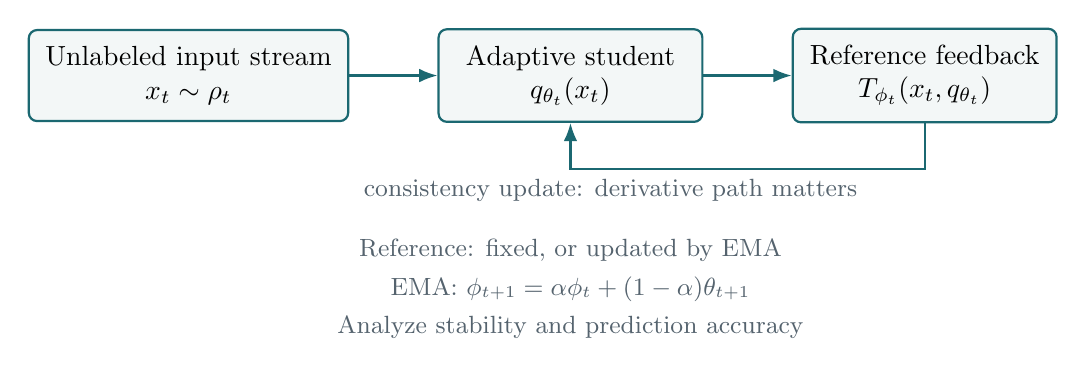
\begin{tikzpicture}[>=Latex,node distance=1.00cm and 1.12cm,
 state/.style={draw=accent,rounded corners=3pt,thick,fill=lightbg,align=center,minimum height=1.05cm,minimum width=3.35cm,inner sep=6pt},
 note/.style={font=\small,align=center,text=muted}]
 \node[state] (stream) {Unlabeled input stream\\$x_t\sim\rho_t$};
 \node[state,right=of stream] (student) {Adaptive student\\$q_{\theta_t}(x_t)$};
 \node[state,right=of student] (teacher) {Reference feedback\\$T_{\phi_t}(x_t,q_{\theta_t})$};
 \draw[->,thick,accent] (stream)--(student);
 \draw[->,thick,accent] (student)--(teacher);
 \draw[->,thick,accent] (teacher.south) |- ++(-3.65,-0.58) -| node[pos=0.20,below,note]{consistency update: derivative path matters} (student.south);
 \node[note,below=1.35cm of student] {Reference: fixed, or updated by EMA\\[3pt] EMA: $\phi_{t+1}=\alpha\phi_t+(1-\alpha)\theta_{t+1}$\\[3pt] Analyze stability and prediction accuracy};
\end{tikzpicture}
\end{center}
\vfill

\newpage
\pagenumbering{arabic}
\begin{abstract}
Test-time adaptation allows a pretrained model to learn from incoming data without additional labels. In idempotent test-time training (IT$^3$), the model's prediction becomes an input to a reference network, creating a feedback loop. The resulting learning dynamics depend on which gradients pass through the reference and whether its parameters remain fixed or follow the adapting model.

This research will analyze how these choices affect stability and prediction accuracy. We will characterize the update fields induced by different gradient paths, study the coupled dynamics of the model and reference, and investigate their behavior under changing input distributions. Mathematical analysis, including local stability and Lyapunov methods, will guide controlled experiments on trained models. The goal is to identify conditions that support stable, useful adaptation and explain when consistency-driven updates improve predictions.
\end{abstract}

\section{Motivation and research question}

\subsection{From stop-gradient to continual adaptation}
Test-time adaptation uses incoming unlabeled data to adjust a model to conditions that may differ from its training environment. A reference network can supply a consistency signal for these updates. How this feedback is differentiated, and how the reference evolves, determine the learner's dynamics.

Stop-gradient leaves forward values intact while removing selected derivative paths. The same forward loss can therefore produce different update fields. Analyses of stop-gradient regression and predictor-based self-distillation provide foundations for studying stationary behavior, convergence, and representation quality \cite{shen2026,peira2026}. We build on these foundations to study prediction-input feedback in IT$^3$ and extensions with a moving reference.

As the input distribution changes, adaptation should improve predictions in the current environment. When earlier environments recur, retention and recovery also become relevant \cite{oclreview2025,clposition2026}. This motivates studying both the immediate effects of feedback-driven updates and their behavior over time.

\subsection{Central question}
\begin{quote}
\itshape How do gradient paths and reference-update timescales shape the stability and predictive performance of test-time adaptation under distribution shift?
\end{quote}

The study evaluates three properties:
\begin{enumerate}
\item \textbf{Self-consistency:} the model approximately satisfies the fixed-point relation used as its adaptation signal.
\item \textbf{Dynamical stability:} trajectories return toward an equilibrium or track a moving solution under the specified update field.
\item \textbf{Predictive quality:} adaptation improves accuracy on the current task and, when tasks recur, preserves performance on previously encountered tasks.
\end{enumerate}
Self-consistency and stability do not by themselves establish predictive accuracy; we will evaluate these properties separately.

\newpage
\section{Existing foundations and the gap to investigate}

\subsection{\texorpdfstring{IT$^3$}{IT3} as a concrete self-referential mechanism}
IT$^3$ trains a dual-input predictor $f_\theta(x,z)$ using both a neutral auxiliary input and the target output as auxiliary input, encouraging $f_\theta(x,0)$ and $f_\theta(x,y)$ to approximate $y$ during supervised pretraining \cite{it3}. At test time, an unlabeled instance $x$ produces a first prediction $q_\theta(x)=f_\theta(x,0)$; feeding this prediction into a reference produces a second prediction. Their discrepancy supplies an adaptation signal.

The literature already includes test-time training with auxiliary self-supervision \cite{sun2020}, online teacher--student adaptation and restoration to source weights \cite{cotta2022,eata2022,rmt2023}, and study of recurring test distributions \cite{petta2024}. Recent preprints also compare fixed and moving teachers and combine EMA with source anchoring \cite{sojka2026,desa2026}. Thus, the generic assertions that ``EMA can be unstable,'' ``retention can fail,'' or ``resetting sometimes helps'' would not form a sufficient new contribution.

Our narrower opportunity is a computation-graph-specific analysis of a \emph{dual-input feedback reference}, followed by a test of whether the resulting field geometry predicts anything meaningful about adaptation or retention. This must be evaluated against the closest teacher--student analyses, not only against generic results on stop-gradient or gradient flow.

\subsection{Which earlier results are inputs, not proposed novelties}
\begin{center}
\small
\begin{tabularx}{\linewidth}{@{}p{0.26\linewidth}X@{}}
\toprule
\textbf{Existing ingredient} & \textbf{Role in the proposed work} \\
\midrule
Stop-gradient lift and semi-gradient fields \cite{shen2026,games2019} & Mathematical language for distinguishing forward values from update fields; not an invention of this project. \\
Self-distillation and PEIRA \cite{peira2026} & Illustrates why equilibrium stability and representation quality must be analyzed separately. \\
IT$^3$ and continual TTA \cite{it3,cotta2022,rmt2023,petta2024} & Concrete adaptive mechanism, implementation constraints, and essential baselines. \\
EMA as coupled dynamics \cite{belay2023} & Motivation for timescale analysis; a spring analogy alone is not a novelty claim. \\
Online learning and shifting distributions \cite{oclreview2025,clposition2026} & Defines evaluation settings and the distinction between present adaptation and retention. \\
\bottomrule
\end{tabularx}
\end{center}

The first task is consequently not to propose another general interpretation of \texttt{detach()}, but to identify a property specific to \emph{prediction-input feedback}, and to determine when that property matters for the behavior of an adaptive learner.

\newpage
\section{A precise learning model}
\label{sec:model}

\subsection{Data, predictions, and model parameters}
Let $x\sim\rho_t$ be a test input, where $\rho_t$ is the input distribution at time $t$. The student and reference share the architecture $f(x,z)$ and have parameter vectors $\theta,\phi\in\R^p$. The auxiliary input $z$ and the model output lie in $\R^d$; $p$ is the number of parameters and $d$ the prediction dimension. Using $0$ to denote the neutral auxiliary signal, define
\begin{equation}
q_\theta(x)=f_\theta(x,0),\qquad
T_\phi(x,z)=f_\phi(x,z),\qquad
r(\theta,\phi;x)=T_\phi(x,q_\theta(x))-q_\theta(x).
\label{eq:residual}
\end{equation}
Thus $q_\theta$ is the student's initial prediction, $T_\phi$ is the reference response, and $r$ measures their disagreement after feeding the prediction into the reference. Our initial smooth model uses the squared discrepancy
\begin{equation}
D_2(\theta,\phi;\rho)=\frac12\E_{x\sim\rho}\norm{r(\theta,\phi;x)}^2,
\label{eq:squared}
\end{equation}
where $\norm{\cdot}$ is the Euclidean norm and $\E$ denotes expectation. The audited IT$^3$ regression implementation uses an absolute discrepancy; we will examine that loss separately using nonsmooth analysis.

During adaptation, the learner observes $x$ but not its correct target $y$. Predictive risk is the expected error against that target:
\begin{equation}
\Risk_t(\theta)=\E_{(x,y)\sim\mu_t}\ell(q_\theta(x),y),\qquad
\rho_t=\text{the input marginal of }\mu_t.
\label{eq:risk}
\end{equation}
Here $\mu_t$ describes input--target pairs, and $\ell$ is a prediction loss, such as squared error. The consistency objective can be estimated from unlabeled inputs; predictive risk is evaluated using held-out labels.

\subsection{Gradient paths and reference inputs}
For the smooth model, assume differentiation may pass through the expectation. Define the student Jacobian $J_q=\partial_\theta q_\theta(x)\in\R^{d\times p}$ and the reference-input Jacobian
\begin{equation}
A_\phi(x,z)=\partial_z T_\phi(x,z),\qquad A=A_\phi(x,q_\theta(x))\in\R^{d\times d}.
\end{equation}
They measure how the student prediction responds to its parameters and how the reference responds to its auxiliary input, respectively. With $\phi$ held fixed, the prediction contributes through both appearances in \eqref{eq:residual}. The chain rule gives
\[
\partial_\theta r=AJ_q-J_q=(A-I)J_q,
\]
where $I$ is the $d\times d$ identity matrix. The resulting student gradient is
\begin{equation}
G_{\mathrm{input}}=\nabla_\theta D_2
=\E_\rho\left[J_q^\top(A-I)^\top r\right].
\label{eq:inputgrad}
\end{equation}
Freezing the reference parameters therefore retains the derivative through its input. If its entire output is instead detached, that output is treated as constant during the backward pass. Only the direct $-q_\theta$ term contributes, yielding the semi-gradient
\begin{equation}
G_{\mathrm{stop}}=-\E_\rho\left[J_q^\top r\right].
\label{eq:stopgrad}
\end{equation}
Both rules use the same forward discrepancy at a shared state. Their gradient difference is
\begin{equation}
G_{\mathrm{input}}-G_{\mathrm{stop}}
=\E_\rho\left[J_q^\top A^\top r\right].
\label{eq:gradientdifference}
\end{equation}
They agree exactly when this expected contribution vanishes. A nonzero $A$ alone does not ensure a difference, since the residual, student Jacobian, and averaging also enter the expression. A gradient-style update moves in direction $-G$.

For repeated updates on the same input, we can also compare \emph{refreshing} the reference input with the current $q_\theta(x)$ against \emph{caching} an earlier prediction $c(x)$. Ordinary differentiation treats the cached value as constant. A straight-through diagnostic can instead retain a cached forward value while prescribing its backward derivative. These controls separate the effect of the supplied value from that of the gradient path.

\subsection{Coupled continuous-time and discrete-time dynamics}
For a fixed reference, $\phi$ remains constant. To study a moving reference, we couple the student update field $G$, initially \eqref{eq:inputgrad} or \eqref{eq:stopgrad}, to a reference that follows the student:
\begin{equation}
\boxed{\quad \dot\theta=-G(\theta,\phi;\rho_t),\qquad
\dot\phi=\frac{\theta-\phi}{\tau},\quad \tau>0.\quad}
\label{eq:jointode}
\end{equation}
Dots denote derivatives with respect to continuous time. The timescale $\tau$ controls the reference's response: larger $\tau$ means slower movement toward the student.

In discrete time, let $n$ index updates, $\eta>0$ be the student learning rate, and $\rho_n$ the input distribution at step $n$. A student-first update followed by exponential moving averaging (EMA) is
\begin{equation}
\theta_{n+1}=\theta_n-\eta G(\theta_n,\phi_n;\rho_n),\qquad
\phi_{n+1}=\alpha\phi_n+(1-\alpha)\theta_{n+1},\quad 0<\alpha<1.
\label{eq:jointdiscrete}
\end{equation}
Larger $\alpha$ retains more of the previous reference; $\alpha=1$ recovers the fixed-reference case. The displayed field uses a population expectation, estimated from the adaptation batch in experiments. Choosing $\alpha=\tau/(\tau+\eta)$ gives $(1-\alpha)/\eta\to1/\tau$ as $\eta\to0$, consistent with \eqref{eq:jointode} under the time scaling $t=n\eta$ and suitable regularity. We will analyze the finite-step map alongside this continuous-time model, with optimizer-state extensions addressed below.

\section{Research questions and theoretical program}
\label{sec:questions}

\subsection{Question I: how do feedback and gradient paths affect adaptation?}
\textbf{Question.} Which properties of the reference-input Jacobian and residual determine whether connecting or stopping the reference-output gradient changes a student update? How does refreshing the reference input affect subsequent updates and predictions?

Using \eqref{eq:gradientdifference} and derivatives of the joint update field, we will derive conditions that predict changes in update direction and subsequent predictions. We will begin with smooth models, then examine piecewise-linear networks and absolute discrepancies. The analysis and experiments will distinguish three outcomes: changes in gradients, changes in parameter steps, and changes in prediction error.

Optimizer state is part of this comparison. For Adam, let $g_n$ be the gradient used at step $n$. Its moment estimates satisfy
\begin{equation}
m_n=\beta_1m_{n-1}+(1-\beta_1)g_n,\qquad
s_n=\beta_2s_{n-1}+(1-\beta_2)g_n^{\odot2}.
\label{eq:adam}
\end{equation}
Here $m_n$ averages past gradients, $s_n$ averages their componentwise squares, and $\beta_1,\beta_2\in[0,1)$ control how much history is retained. The notation $g_n^{\odot2}$ denotes componentwise squaring.

Identical weights can therefore produce different parameter steps when moment estimates or step counts differ. We will match weights, optimizer state, and step counts when isolating gradient-path effects, and use separate controlled comparisons to measure the contribution of optimizer history.

\subsection{Question II: can a useful equilibrium be locally stable?}
\textbf{Question.} Under what structural conditions does the coupled learner converge to a \emph{nondegenerate, prediction-relevant} equilibrium? Can different backward rules or EMA timescales change the linear stability classification?

Suppose $\rho$ is fixed and $(\theta^*,\phi^*)$ is an equilibrium of \eqref{eq:jointode}. Then $\theta^*=\phi^*$, and $G(\theta^*,\theta^*;\rho)=0$. Write $u=\theta-\theta^*$ and $v=\phi-\phi^*$, and define
\begin{equation}
H=\partial_\theta G(\theta^*,\phi^*;\rho),\qquad
K=-\partial_\phi G(\theta^*,\phi^*;\rho).
\end{equation}
The linearization is
\begin{equation}
\frac{d}{dt}\begin{pmatrix}u\\v\end{pmatrix}
=\underbrace{\begin{pmatrix}-H&K\\ \tau^{-1}I&-\tau^{-1}I\end{pmatrix}}_{M_\tau}
\begin{pmatrix}u\\v\end{pmatrix}.
\label{eq:blockM}
\end{equation}
We will examine how the spectrum of $M_\tau$ depends on the feedback Jacobian and reference timescale. For a Hurwitz linearization, a local quadratic Lyapunov certificate can be constructed from
\begin{equation}
M_\tau^\top P+PM_\tau=-Q,\qquad P\succ0,\quad Q\succ0.
\label{eq:lyapeq}
\end{equation}
This classical construction certifies local stability under the usual smoothness hypotheses; using it alone is not a novel result. What may be valuable is a structural condition, verifiable from a trained model's dual-input geometry, that predicts a stability boundary or excludes a failure mode.

The equilibrium must also be \emph{useful}. An exactly stable zero predictor is not a success for an adaptation problem. We will therefore require a nonconstant baseline prediction rule, separate evaluator labels, and a clear account of which parameter directions affect predictions. In overparameterized networks, neutral parameter directions may prevent strict stability in the full weight space even when the output behavior is well controlled. Observable or quotient-space stability may be the appropriate statement.

\subsection{Question III: what happens when the data distribution moves?}
\textbf{Question.} If the input distribution changes over time, can the student--reference system track a useful equilibrium family? How does tracking error depend on drift speed, teacher lag, and choice of backward rule?

For fixed $\rho$, even an ordinary student gradient field need not decrease $D_2$ because the reference moves. Direct differentiation gives
\begin{equation}
\frac{d}{dt}D_2(\theta,\phi;\rho)
=-\norm{\nabla_\theta D_2}^2
+\frac1\tau\ip{\nabla_\phi D_2}{\theta-\phi}
\qquad (G=G_{\mathrm{input}}).
\label{eq:Ddot}
\end{equation}
The second term has no fixed sign. With a stopped-output field, the first term becomes $-\ip{\nabla_\theta D_2}{G_{\mathrm{stop}}}$. Under distributional drift there is also explicit time dependence in the expectation, where differentiability is available; abrupt changes instead require a switching or jump analysis. Hence an observed decrease in consistency at one instant is not a general Lyapunov property of the coupled process.

A more relevant objective is often a \emph{tracking} certificate. Let $z=(\theta,\phi)$ and let $z^*(t)$ denote a justified desired solution, not merely an arbitrary stationary point. For a candidate $V(z,t)$ measuring $e=z-z^*(t)$, the derivative includes the motion of the target:
\begin{equation}
\dot e=F(z;\rho_t)-\dot z^*(t),\qquad
\dot V=\partial_tV+\nabla_zV^\top F(z;\rho_t).
\label{eq:tracking}
\end{equation}
A possible theorem target is an input-to-state-type estimate
\begin{equation}
\norm{e(t)}\ \leq\ C e^{-\gamma t}\norm{e(0)}
+\frac{C}{\gamma}\sup_{0\leq s\leq t}\norm{\dot z^*(s)}
\label{eq:trackbound}
\end{equation}
under explicit uniform stability and regularity conditions. This is a \emph{target form}, not a theorem already established for IT$^3$. In particular, stable Jacobians at individual times do not imply stability under arbitrary switching; a common metric, slow-variation condition, or other suitable hypothesis is needed. Translating state tracking into predictive-risk tracking additionally requires an alignment between the desired state and the unknown labels.

\subsection{Question IV: can stability explain retention or recovery?}
\textbf{Question.} When domains recur, which parts of the learner's state preserve information relevant to a return task? Does a reference or optimizer history improve \emph{readaptation}, rather than merely delay change?

We will first distinguish compatible distribution shifts (a fixed underlying label rule with changing input marginals) from genuinely conflicting tasks (different labels for indistinguishable inputs). The latter cannot generally be resolved from unlabeled observations alone. For compatible recurring domains, controlled streams such as $A\to B\to A$ can test whether student weights, reference weights, or optimizer history influence later recovery. However, a changed update direction does not by itself demonstrate useful memory. We will require matched baselines, equal adaptation budgets, held-out labels for evaluation only, and evidence that any benefit is specifically attributable to the earlier visit rather than an unrelated intervening update.

\section{Accuracy, information, and the meaning of forgetting}
\label{sec:accuracy}

\subsection{Why unlabeled consistency cannot certify accuracy in general}
Let $p\in\R^n$ be current predictions on a set of evaluator inputs, $d\in\R^n$ the change after adaptation, and $y\in\R^n$ the hidden targets. For squared prediction error,
\begin{equation}
\Risk(p+d)-\Risk(p)
=\frac1n\left(\norm{d}^2-2\ip{y-p}{d}\right).
\label{eq:riskchange}
\end{equation}
Thus the update improves accuracy exactly when $\ip{y-p}{d}>\norm{d}^2/2$. The learner can compute $p$ and $d$, but generally does not know $y-p$. A small consistency residual, a stable learning trajectory, or a particular Jacobian sign cannot determine the sign of \eqref{eq:riskchange} without further assumptions.

The technical backbone gives a sharp compatible linear illustration. Let $S$ contain retained source-feature rows and $X$ current unlabeled rows. Choose an update $h$ such that $Sh=0$ yet $Xh\ne0$. Two possible label coefficients $w+h$ and $w-h$ agree on all the retained labels $Sw$ and produce the same unlabeled current inputs. Starting from $p=Xw$ and updating by $d=Xh$ achieves zero error in one possible world and increases error in the other. This is an \emph{identifiability obstruction}: no deterministic rule seeing only the shared information can certify improvement in both worlds. We retain it as a baseline limitation, not as a proposed general impossibility theorem.

\subsection{What additional evidence could make guarantees possible?}
An instructive positive baseline arises when independently justified information restricts the true linear coefficient to a known compact convex set $\mathcal C$ that preserves selected source predictions. Let $Y=X\mathcal C$ be the corresponding set of possible current predictions. The Euclidean projection $z=\Proj_Y(p)$ satisfies, for every possible true $y\in Y$,
\begin{equation}
\norm{z-y}^2\leq\norm{p-y}^2-\norm{p-z}^2.
\label{eq:projection}
\end{equation}
The conclusion relies on the feasibility set containing the truth; unlabeled inputs alone do not supply this fact. Projection-based safe-prediction results are established prior work \cite{li2017}. Their role here is to clarify \emph{which information is missing} from an unconstrained consistency learner and to motivate assumptions that are defensible in future models.

We do not intend to claim that IT$^3$ itself implements \eqref{eq:projection}. Instead, the analytic challenge is to characterize a weaker, realistic condition connecting consistency updates to trustworthy predictions: for example, calibrated source information, a restricted shift family, or a model-based relation between reference fixed points and true labels. An assumption that already encodes the correct answer would not be satisfactory.

\subsection{Retention must be assessed at matched adaptation quality}
For two distributions $\mu_A$ and $\mu_B$, define $\Risk_A$ and $\Risk_B$ as in \eqref{eq:risk}. During adaptation to $B$, it is possible that $\Risk_B$ decreases while $\Risk_A$ increases, even when the dynamics are stable and both tasks are compatible. This does not yet establish catastrophic failure: the old task may no longer be relevant, or the observed retention may merely reflect slower adaptation.

The evaluation should report both current-task performance and previously relevant performance. When comparing retention interventions, it should also compare old-task error \emph{at matched current-task risk}, not solely at a common iteration count. If a returning domain matters, recovery should be defined operationally, for instance as the number of fresh return samples or updates needed to regain a target level of held-out performance, under a shared evaluation protocol.

\section{Research plan and empirical design}
\label{sec:work}

\subsection{Work package A: establish the exact algorithm and graph}
We begin with one reproducible regression-style IT$^3$ implementation and declare: its two inputs and neutral signal; pretrained checkpoint; trainable parameters and reference copy; loss (absolute or squared); backward rule; optimizer state; and the ordering of student and EMA updates. We will verify automatic derivatives against the derived $J_q$ and $A$ formulas. In the two-update setting, we will compare four controlled forward/backward variants, with identical initialization and optimizer history, and record precisely when their second gradients and outputs begin to differ.

\textbf{Deliverable:} a tested computation-graph specification and a reproducible first-order mechanism result. \textbf{Rejection condition:} if a proposed distinction disappears when the actual loss and official graph are used, or depends only on mismatched optimizer states, we will narrow or abandon that claim.

\subsection{Work package B: build a genuine dynamics result}
We will analyze low-dimensional smooth dual-input models where the source solution gives distinct, correct predictions. The first objective is a nontrivial stability comparison of the two backward rules for the same forward architecture and teacher update; the second is to identify assumptions that can be checked or at least measured in a trained model.

The technical backbone already contains a constructed local stability distinction, as well as counterexamples to overly broad monotonicity claims. These examples are useful proof tests, but they do not establish generic properties of pretrained neural networks. We will check whether the mechanism persists when the reference-input map is close to an idempotent projection, when parameter directions commute or fail to commute, and when the loss is nonsmooth. If a useful certificate exists, we will specify the metric, basin, equilibrium assumptions, and whether it controls parameters or predictions.

\textbf{Deliverable:} one exact theorem with transparent assumptions, or a counterexample sharply delimiting a tempting extension. \textbf{Rejection condition:} if the result is only a generic linear-system fact, relies on a planted correct equilibrium without empirical relevance, or reduces to a change of time scale, it is not sufficient as a standalone contribution.

\subsection{Work package C: connect stability to a changing environment}
Only after the fixed-distribution mechanism is understood will we introduce a controlled covariate shift $\rho_t$ and then recurring domains. The initial target is a restricted family with a shared, known-for-evaluation labeling rule; a separate conflicting-label experiment will illustrate the information limit. We will seek tracking estimates under drift conditions that are explicitly related to the student--reference field, rather than assuming contraction as a free property.

For recurrence experiments, compare a return to $A$ after an earlier visit to $A$ with a matched return after a different earlier domain $C$, passing through the same bridge $B$. Keep the bridge duration, evaluation inputs, step counter, training budget, and randomization aligned. Include no adaptation, fresh optimizer state, carried optimizer state, fixed reference, moving EMA, and a suitable established restoration or anchoring baseline. Track both the pre-return state and the post-return response. A reported memory benefit must survive the controls that remove earlier-visit information without changing other resources.

\textbf{Deliverable:} a prediction about tracking or return adaptation that can be independently tested. \textbf{Rejection condition:} a change in trajectories without a reproducible benefit to held-out accuracy, or an effect also produced by a neutral earlier history, will not be interpreted as meaningful retention.

\subsection{Work package D: selective extension to the actual optimizer}
If the graph and dynamics studies suggest a useful principle, we will test whether optimizer memory, normalization state, or EMA schedule changes its predictions. Since the local implementation may reset student weights while retaining Adam moments, the state of the adaptation algorithm must be modeled as $(\theta,\phi,m,s,n)$ rather than just $(\theta,\phi)$. This branch is conditional: a striking dependence on optimizer history is not enough; it must survive controls with matched parameters, counters, and adaptation budgets and must reveal an effect not already covered by continual-learning optimizer-state work \cite{kang2024,petta2024}.

\section{Evaluation protocol and criteria for success}

\subsection{A deliberately small progression of settings}
\begin{enumerate}
\item \textbf{Analytic models.} Linear or low-dimensional smooth dual-input predictors with transparent covariance and reference-input derivatives. Use exact eigenvalue tests, small-time calculations, and, where appropriate, Lyapunov equations.
\item \textbf{Trained synthetic networks.} Nonconstant regression tasks with separately held-out labels and several independent initializations. Record the actual residual and Jacobian geometry rather than assuming the trained network resembles the analytic example.
\item \textbf{Specified IT$^3$ regression implementation.} Reproduce its particular loss, auxiliary-input convention, frozen-reference pathway, and optimizer policy before making claims about practical behavior. The technical backbone's exploratory surrogates are not substitutes for this reproduction.
\item \textbf{Continuous and recurring streams.} Start with one fixed labeling function and changing covariate distributions, then controlled recurring domains. Only later investigate label changes that create a fundamentally different identification problem.
\end{enumerate}

\subsection{Quantities to record}
The primary outcome is held-out current-task risk, measured both before and after each adaptation batch. We will additionally track consistency discrepancy, prediction variance or other collapse indicators, reference lag $\norm{\theta-\phi}$, finite-step perturbation amplification, and return-domain error or recovery. Whenever a Jacobian spectrum is reported, we must distinguish a true equilibrium from a moving checkpoint: positive instantaneous eigenvalues at nonstationary points are diagnostics, not asymptotic stability certificates. For nonsmooth absolute losses, we will distinguish the literal discrete algorithm from any ODE or differential-inclusion approximation, and verify step-size sensitivity before asserting a continuous-time interpretation.

\subsection{Prospective comparison rather than retrospective explanation}
Experiments will use fixed data splits, predetermined model configurations, paired seeds, and explicit success thresholds before evaluating new outcomes. The comparison must separate (i) the effect of refreshing a reference input, (ii) the effect of propagating its derivative, (iii) movement of reference parameters, and (iv) optimizer memory. Matching only forward weights is insufficient when an adaptive optimizer carries hidden state. Failures of predicted stability ordering, collapse prevention, numerical robustness, or accuracy improvement will be reported as outcomes; they will not be repaired by silent changes to step sizes, models, or evaluation populations.

\section{Expected contribution, risks, and decisions}

\subsection{A realistic hierarchy of possible contributions}
The project has several scientifically useful endpoints, with different novelty requirements:
\begin{enumerate}
\item \textbf{Mechanism theorem.} A precise structural condition, specific to prediction-fed reference models, that distinguishes backward rules or predicts a bounded stability regime beyond generic Lyapunov linearization.
\item \textbf{Tracking or retention result.} A theorem or counterexample stating when a learner can follow a changing solution under explicitly justified task assumptions, with a corresponding observable test.
\item \textbf{Validated computational mechanism.} A reproducible causal comparison on a faithful adaptation graph, showing when prediction-input feedback or retained optimizer state meaningfully changes adaptation and where the effect fails.
\end{enumerate}
No one item is guaranteed. A classical certificate rederived for an arbitrary field, another demonstration of EMA instability, or an unlabeled loss reduction without a measurable accuracy consequence is not an adequate standalone contribution.

\subsection{Principal risks and how they shape scope}
\textbf{Incorrect objective alignment.} Self-consistency may stabilize an inaccurate predictor. We will never infer accuracy from discrepancy alone; evaluator labels and explicit identifiability assumptions are necessary.\\
\textbf{Unrealistic geometry.} Constructed rotating reference-input Jacobians may be absent in pretrained idempotent networks. We will measure the geometry of trained models and abandon assumptions that fail their test.\\
\textbf{Nonsmoothness and discretization.} Actual absolute-loss and ReLU/Adam implementations can exhibit finite-step behavior not captured by a smooth ODE. Those systems will be studied directly or excluded from a smooth theorem's scope.\\
\textbf{Overlapping prior work.} Continual TTA already contains moving teachers, restoration, replay, recovery analyses, and parameter-memory mechanisms. A novelty audit focused on the exact graph, information budget, and evaluation protocol is part of every work package.\\
\textbf{Insufficient evidence.} Preliminary synthetic patterns may be initialization-sensitive or fail independent tests. A negative or bounded result can still sharpen the thesis, but will not be advertised as a successful adaptation method.

\subsection{Proposed sequence of decisions}
\begin{center}
\small
\begin{tabularx}{\linewidth}{@{}p{0.19\linewidth}p{0.37\linewidth}X@{}}
\toprule
\textbf{Stage} & \textbf{Question to resolve} & \textbf{Go / narrow decision}\\
\midrule
Graph & What exact update does the selected IT$^3$ implementation perform? & Derivatives and state transitions independently reproducible.\\
Geometry & Is a noncollapsed useful state stable, or can the backward rule change its classification? & Condition survives checks beyond a planted toy example.\\
Drift & Can a measurable model property support a tracking bound? & A stated hypothesis links equilibrium motion, feedback, and error.\\
Recurrence & Does earlier history help readaptation at controlled current-task quality? & Benefits survive matched histories and independent test data.\\
\bottomrule
\end{tabularx}
\end{center}

The first group discussion should choose which of the first two stages is most promising as a narrow theorem target, and which practical IT$^3$ implementation should be treated as authoritative. A move to continual-learning claims should follow, not precede, that decision.

\section{Conclusion}
The proposed pivot preserves the most useful lesson of Detach research: a training objective's forward value does not determine its update dynamics. IT$^3$ makes this lesson concrete because a student prediction enters a reference network whose parameters may be frozen or slowly moving, while derivative paths can be independently connected or blocked. Our aim is to understand that feedback mechanism with dynamical-systems tools, then establish what additional assumptions are required for stability to say anything about useful online predictions.

The near-term goal is intentionally modest: a fully specified computation graph, a sharp analytic question about its coupled dynamics, and a reproducible experiment capable of refuting the proposed mechanism. The longer-term ambition is to relate such a result to tracking and retention in changing environments, without conflating consistency, convergence, and predictive correctness.

\vspace{0.6em}
\noindent{\small\itshape Research developed through discussion and collaboration with a fellow master's student from the Faculty of Data and Decision Sciences. The longer technical record is preserved separately as \emph{Research Backbone} and is not part of the submission argument.}

\begin{thebibliography}{99}\small\setlength{\itemsep}{2pt}
\bibitem{it3} N. Durasov et al., ``IT$^3$: Idempotent Test-Time Training,'' \emph{International Conference on Machine Learning}, 2025.
\bibitem{shen2026} M. W. Shen et al., ``How I Learned to Stop Worrying and Love StopGrads: Stationarity, Convergence, and a Case Study on Flow Map Learning,'' arXiv:2609.16222, 2026.
\bibitem{peira2026} M. Arbel, B. Terver, and J. Ponce, ``PEIRA: Learning Predictive Encoders through Inter-View Regressor Alignment,'' arXiv:2605.17671, 2026.
\bibitem{games2019} L. Letcher et al., ``Differentiable Game Mechanics,'' \emph{Journal of Machine Learning Research}, 2019.
\bibitem{sun2020} Y. Sun et al., ``Test-Time Training with Self-Supervision for Generalization under Distribution Shifts,'' \emph{ICML}, 2020.
\bibitem{cotta2022} Q. Wang et al., ``Continual Test-Time Domain Adaptation,'' \emph{CVPR}, 2022.
\bibitem{eata2022} S. Niu et al., ``Efficient Test-Time Model Adaptation without Forgetting,'' \emph{ICML}, 2022.
\bibitem{rmt2023} M. Doebler, R. A. Marsden, and B. Yang, ``Robust Mean Teacher for Continual and Gradual Test-Time Adaptation,'' \emph{CVPR}, 2023.
\bibitem{petta2024} T.-H. Hoang, D. M. Vo, and M. N. Do, ``Persistent Test-Time Adaptation in Recurring Testing Scenarios,'' \emph{NeurIPS}, 2024.
\bibitem{sojka2026} D. Sojka et al., ``Rethinking the Teacher--Student Framework for Test-Time Adaptation,'' preprint, arXiv:2609.02507, 2026.
\bibitem{desa2026} A. Belal et al., ``DESA-TTA: Dynamic EMA and Source Anchoring for Test-Time Adaptation,'' preprint, arXiv:2609.01795, 2026.
\bibitem{belay2023} J. Patsenker, H. Li, and Y. Kluger, ``Exponential Weight Averaging as Damped Harmonic Motion,'' ICML Workshop, 2023.
\bibitem{li2017} Y.-F. Li, H.-W. Zha, and Z.-H. Zhou, ``Learning Safe Prediction for Semi-Supervised Regression,'' \emph{AAAI}, 2017.
\bibitem{kang2024} L. Kang and W. S. Lee, ``Continual Learning of Numerous Tasks from Long-tail Distributions,'' arXiv:2404.02754, 2024.
\bibitem{oclreview2025} S. A. Bidaki et al., ``Online Continual Learning: A Systematic Literature Review of Approaches, Challenges, and Benchmarks,'' arXiv:2501.04897, 2025.
\bibitem{clposition2026} ``Forgetting is not Catastrophic, Our Benchmarks Are,'' position manuscript supplied for group reading, 2026.
\end{thebibliography}
\end{document}
